\documentclass[pdf]{beamer}
\usepackage[utf8]{inputenc}
\usepackage{graphicx}

\usetheme{warsaw}
\mode<presentation>{}

\title{Projet 2 : concevoir un haut-parleur}
\subtitle{Pré-jury}
\author{Groupe 115.3}
\date{\today}

\begin{document}

\begin{frame}
	\titlepage
\end{frame}

\begin{frame}
	\frametitle{Etat d'avancement du projet}	
	% Contenu
\end{frame}

\begin{frame}
	\frametitle{Recherche documentaire}
	\framesubtitle{La contre-réaction (ou contre réaction négative)}
	
	
	
\end{frame}

\begin{frame}
	\frametitle{Recherche documentaire}
	\framesubtitle{La distorsion}
	% Contenu
\end{frame}
	
\begin{frame}
	\frametitle{Approximation de la fréquence de coupure}
	% Contenu
\end{frame}

\begin{frame}
	\frametitle{Modélisation du filtre passe-haut}
	% Contenu
\end{frame}

\begin{frame}
	\frametitle{Modélisation du filtre passe-bas}
	% Contenu
\end{frame}

\begin{frame}
	\frametitle{Dimensionnement du haut-parleur}
	% Contenu
\end{frame}

\begin{frame}
	\frametitle{Dimensionnement des bobines}
	

	\center{
\begin{minipage}{0.5\linewidth}
{\center{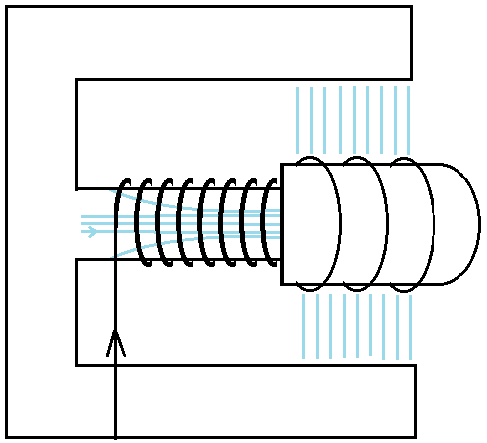
\includegraphics[scale=0.2]{hautparleur.png}}}
\end{minipage}\hfill
\begin{minipage}{0.5\linewidth}
\center{La bobine fixe joue un rôle d'électroaimant. Dans des conditions idéales, le champ total crée est $B = \unit{0.1143}{\tesla}$}
\end{minipage}
\\

 \vspace{4\baselineskip}
	
\paragraph{\textbf{Tableau récapitulatif}}
\small{\begin{center}
\begin{tabular}{c|c|c|c|c|c}
$$ & $N$ & $I$ & $R$ & $L$ & $L_{fil}$ \\
\hline
$Bobine fixe$ & $400$ & $\unit{2.5}{\ampere}$ & \unit{5.904}{\ohm} & $\unit{7.6403 \cdot 10^{-3}}{\henry}$ & $\unit{32.8}{\meter}$\\
\hline
$Bobine mobile$ & $ 70 $ & $\unit{0.1667}{\ampere}$ & $\unit{2.38}{\ohm}$ & $\unit{0.0134}{\henry}$ &\unit{12.6}{\meter}$\\
\end{tabular}

	\end{center}}
	}\\


\end{frame}

\end{document}
